\chapter{Background and eBPF architecture}
\label{ch:background-related-work}

\section{Linux Kernel Observability}
\label{sec:linux-kernel-observability}

Runtime monitoring requires evidence about operations while they are being
executed. Application logs describe domain-specific actions, but their content
depends on what each application chooses to record. The Linux kernel offers a
complementary observation layer because it mediates process creation,
credential changes, file access, memory management, inter-process
communication, and other security-relevant operations. Kernel observability is
therefore useful when behaviour crosses application boundaries or is not
represented consistently in application logs
\cite{linux_tracing_index,gbadamosi2024ebpf}.

Linux does not expose all runtime activity through one universal event source.
Instead, it provides instrumentation points at different layers of kernel
execution. Each mechanism determines when monitoring code runs, which context
is available, and how strongly the observation depends on kernel internals.

\medskip
\noindent\textbf{System-call observation.}
A system call is the controlled interface through which a user-space process
requests a service from the kernel. It is not itself an instrumentation
mechanism. Monitoring systems commonly observe this boundary through
system-call tracepoints, such as entry and exit events. An entry event exposes
the requested operation and its original arguments, whereas an exit event
exposes the returned result. Correlating the two can distinguish an attempted
operation from one that completed successfully. This view is broad and
process-oriented, but it remains close to the user-space request: one system
call may traverse several internal functions, and its original arguments may
not identify the final kernel object or security decision
\cite{linux_tracepoints,linux_tracing_index}.

\medskip
\noindent\textbf{Tracepoints and raw tracepoints.}
A tracepoint is a static observation point deliberately inserted into the
kernel source by kernel developers. It has a name, belongs to an event
category, and defines the data made available when that point is reached. A
tracepoint remains inactive until a tracing component is attached to it. In an
eBPF-based monitor, this component is an eBPF program loaded from user space
and attached to the selected tracepoint. Each time kernel execution reaches
that point, the kernel invokes the attached program and provides a
tracepoint-specific context containing the declared event fields.

A regular tracepoint gives the eBPF program a structured event context whose
layout follows the format exported for that tracepoint. A raw tracepoint refers
to the same underlying kernel instrumentation site, but exposes the original
arguments passed by the kernel to that site with less intermediate
transformation. This reduces preparation performed before the eBPF program
runs, while requiring the program to know how each raw argument must be
interpreted. Tracepoints are therefore explicit and comparatively stable
observation points, whereas raw tracepoints trade some of that abstraction for
more direct access to the underlying arguments. Both mechanisms are limited to
the tracepoints actually provided by the target kernel
\cite{linux_tracepoints,linux_libbpf_program_types}.

\medskip
\noindent\textbf{Kprobes and kretprobes.}
A kprobe is a dynamic probe placed at a selected kernel instruction at run
time. Monitoring tools usually identify that instruction through the symbol of
a kernel function and place the probe at its entry. Unlike a tracepoint, the
observation point does not need to have been prepared explicitly by the kernel
developer. When execution reaches the probed instruction, the kernel
temporarily transfers control to the probing infrastructure, which invokes the
attached eBPF program before normal execution continues. The program receives
a snapshot of the processor-register state. Function arguments are not
presented as a tracepoint-specific event structure; they must be recovered from
the appropriate registers according to the architecture and calling
convention.

A kretprobe observes the corresponding function-return path. It causes an
attached program to run when an invocation of the probed function finishes and
makes the return value available through the register context. A kprobe can
therefore describe the operation requested at function entry, while a
kretprobe can reveal the result produced at function exit. Entry and return
records are separate observations: when both the original arguments and the
result are required in one logical event, the monitoring system must save the
entry data and correlate it with the return observation, commonly by using the
current thread identity.

Kprobes and kretprobes provide access to functions for which no tracepoint
exists, but this flexibility increases coupling to kernel implementation
details. A renamed or inlined function, a changed signature, a different
calling convention, or an unavailable symbol can invalidate the attachment or
the argument-decoding logic. They are therefore powerful dynamic mechanisms,
but generally require more target-specific validation than tracepoints
\cite{linux_kprobes}.

\medskip
\noindent\textbf{Linux Security Module hooks.}
The \gls{lsm} framework inserts security mediation points into kernel
operations involving files, credentials, processes, sockets, and other
protected objects. At these points, registered security modules can inspect an
operation and, for hooks with authorisation semantics, permit or reject it.
Observing an LSM-related function can therefore expose a resolved kernel object
and the security-relevant stage of an operation, rather than only the original
system-call request. Two concepts should not be confused: an LSM hook is the
kernel mediation point, while an eBPF LSM program is one possible program type
for attaching logic to supported hooks. On kernels where that program type is
unavailable or unsuitable, monitoring tools may instead observe the
corresponding security function through a kprobe. An entry-side observation
still does not necessarily reveal the final outcome; when the result matters,
it must be obtained from a compatible return-side observation
\cite{linux_lsm_development,linux_libbpf_program_types,linux_kprobes}.

\begin{table}[H]
    \centering
    \footnotesize
    \setlength{\tabcolsep}{5pt}
    \renewcommand{\arraystretch}{1.18}
    \label{tab:kernel-observation-sources}

    \begin{tabularx}{\textwidth}{
        @{}
        >{\raggedright\arraybackslash}p{0.18\textwidth}
        >{\raggedright\arraybackslash}p{0.31\textwidth}
        >{\raggedright\arraybackslash}X
        @{}
    }
        \toprule
        \textbf{Observation source} &
        \textbf{Information exposed} &
        \textbf{Main trade-off} \\
        \midrule

        System-call tracepoint &
        Arguments at entry or return value at exit. &
        Broad process visibility, but limited insight into internal kernel
        processing and resolved objects. \\

        Kernel tracepoint &
        Structured fields defined for a specific kernel event. &
        Clear semantics and simple decoding, but only where a suitable
        tracepoint is available. \\

        Raw tracepoint &
        Original tracepoint arguments with minimal preprocessing. &
        More direct access, but requires kernel-aware argument decoding. \\

        Kprobe / kretprobe &
        Register state at function entry or return. &
        Flexible placement, but stronger dependence on kernel symbols,
        signatures and calling conventions. \\

        LSM-related hook &
        Security context, resolved objects and mediation stage. &
        Rich security semantics, but attachment and result visibility depend
        on target-kernel support. \\

        \bottomrule
    \end{tabularx}
    \caption[Observation sources for eBPF runtime monitoring]
    {Comparison of the principal observation sources relevant to
    eBPF-based runtime monitoring
    \cite{linux_tracepoints,linux_kprobes,linux_lsm_development,
    linux_libbpf_program_types}.}
\end{table}

\medskip
\noindent\textbf{The role of eBPF.}
eBPF is the execution facility attached to an observation point, not a
replacement name for the observation point itself. The selected hook causes an
eBPF program to run and determines the context received by that program. The
program can then extract selected fields, apply an early filter, update maps,
or submit an event to user space. Consequently, ``tracepoint'', ``kprobe'',
``LSM hook'', and ``eBPF program'' describe different parts of the same
monitoring path \cite{linux2024ebpfuserspaceapi,linux_libbpf_program_types}.

These mechanisms are complementary. System-call describe requests
and results at the user--kernel boundary; general tracepoints expose
kernel-defined events; kprobes and kretprobes provide dynamic access to
function entry and return; and LSM-related hooks expose security mediation
points. A runtime monitor combines them according to the required semantics,
available target-kernel features, and acceptable coupling to kernel internals.
The engineering objective is to select observation points that provide sufficient and
reliable evidence for the intended security analysis
\cite{linux_tracing_index,her2025ebpfsecuritytools}.

\section{eBPF Fundamentals}
\label{sec:ebpf-fundamentals}

\gls{ebpf} is a modern technology that makes the Linux kernel programmable at
runtime. It allows small programs to be loaded from user space and executed
inside the kernel when a selected event occurs. Before execution, the kernel
verifies that each program respects the safety constraints associated with its
program type and intended attachment point
\cite{rfc9669_bpf_isa,linux2024ebpfuserspaceapi}.

This approach makes it possible to extend kernel behaviour without modifying
the kernel source or developing a traditional kernel module for each new
functionality. eBPF programs can be loaded, replaced, and specialised for
different purposes, including system observability, performance analysis,
network processing, and security. Its principal benefit is therefore
controlled programmability: functionality can be introduced close to the
kernel operations of interest while remaining subject to verification and
well-defined execution constraints
\cite{gbadamosi2024ebpf,linux2026ebpfverifier}.

\subsection{Execution Model, Verifier and JIT Compilation}
\label{subsec:ebpf-execution-verifier-jit}

An eBPF program is compiled into instructions for the BPF virtual machine and
submitted to the kernel through the BPF user-space interface. The instruction
set defines general-purpose registers, a bounded stack, arithmetic and branch
instructions, memory operations, and calls to kernel-provided functions. The
program does not execute as unrestricted kernel code: its available context,
memory accesses, and callable functions depend on its program type
\cite{rfc9669_bpf_isa,linux_bpf_helpers}.

Because the programs described above are loaded from user space but execute
inside the kernel, they cannot be allowed to run without first establishing
that they respect the kernel's safety constraints. An unsafe memory access or
an invalid operation in this context could affect the stability and security of
the entire system. Linux addresses this requirement through the eBPF verifier,
the kernel component responsible for deciding whether a submitted program can
be accepted for execution. Rather than trusting the program, the verifier
analyses it during the loading process and before permitting its execution; a
program that does not satisfy the required safety conditions is rejected and
never executed.

The verifier performs a path-sensitive static analysis of the program's control
flow. It follows the possible execution paths while tracking the state of
registers and stack locations, distinguishing scalar values from different
classes of pointers, checking memory bounds and alignment, and validating the
arguments supplied to helper functions. Paths that may access invalid memory,
use uninitialised values, or leave kernel-managed resources unreleased are
rejected. To avoid analysing equivalent situations repeatedly, the verifier
uses state pruning: when a previously accepted verifier state already covers a
new state reached at the same instruction, the redundant path does not need to
be explored again \cite{linux2026ebpfverifier,gershuni2019prevail}.

Verification is a necessary safety gate, not a proof that a program implements
the intended monitoring semantics. A verifier-accepted program may still read
the wrong field, emit an incomplete event, or encode data inconsistently with
its user-space decoder. Conversely, semantically reasonable source code may be
rejected because the verifier cannot establish the required safety properties
for a particular kernel. Verifier behaviour is therefore both a security
mechanism and a practical compatibility constraint
\cite{linux2026ebpfverifier,linux_bpf_design_qa}.

Once the verifier accepts a program, the kernel may pass its eBPF instructions
to an architecture-specific \gls{jit} compiler. The compiler translates the
verified eBPF bytecode into native machine instructions for the host
architecture. The resulting native code can then be executed directly whenever
the program is invoked, avoiding the overhead of processing the eBPF
instructions individually at each execution
\cite{linux_bpf_execution_modes,linux_bpf_jit_sysctl}.

\begin{figure}[H]
    \centering

    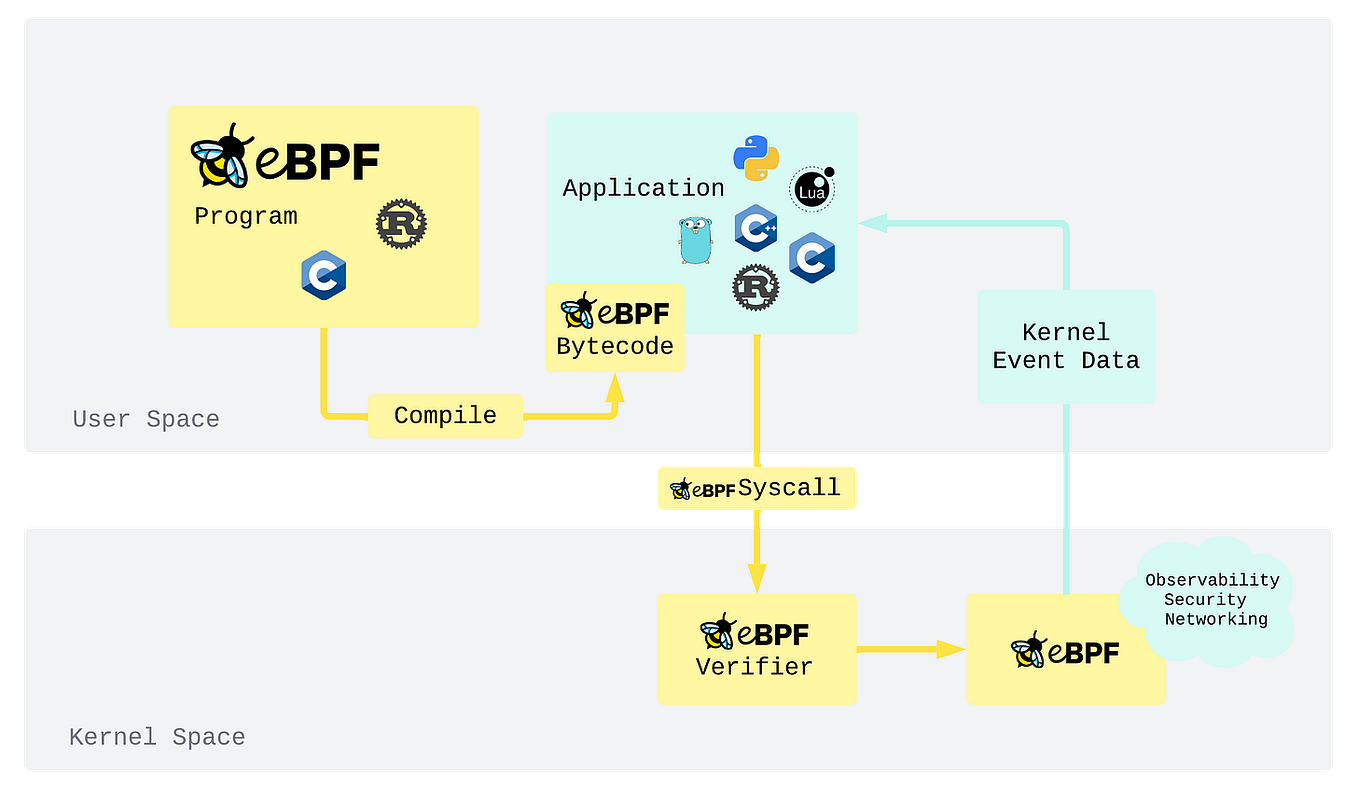
\includegraphics[
        width=0.90\textwidth,
        height=0.65\textheight,
        keepaspectratio
    ]{figures/chapter2/eBPF-schema.png}

    \caption[High-level eBPF execution workflow]
    {High-level eBPF execution workflow.}

    \label{fig:ebpf-execution-workflow}
\end{figure}

JIT compilation does not alter the functionality authorised by the verifier.
The translation is performed only after verification and preserves the
semantics of the accepted eBPF program. Its availability depends on the host
architecture, the kernel build configuration, and the runtime JIT settings.

This completes the basic eBPF execution path considered here. A program is
compiled into eBPF instructions, submitted to the kernel, analysed by the
verifier and, if accepted, translated into native machine code and executed
whenever its associated hook or execution context is invoked
\cite{gbadamosi2024ebpf}.

\subsection{Hook Selection and Event Semantics}
\label{subsec:ebpf-hook-selection-event-semantics}

An eBPF program type defines the execution contract enforced by the kernel,
including the expected context, available helpers, and permitted return
semantics. The hook instead identifies the event or kernel execution point
that triggers the program, while the attachment mechanism binds the loaded
program to a compatible hook. These concepts are related, but they are not
interchangeable
\cite{linux_libbpf_program_types,linux_bpf_helpers}.

The selected observation point determines not only when an eBPF program runs,
but also the meaning of the resulting event. A system-call entry hook captures
the operation requested by a process and its original arguments. A later
tracepoint, dynamic probe, or LSM-related hook may expose kernel-resolved
objects or the security mediation stage of the operation. An exit or
return-side observation can instead reveal whether the operation completed
successfully
\cite{linux_tracepoints,linux_kprobes,linux_lsm_development}.

These observations represent different stages of the same kernel execution
path and should therefore be considered complementary rather than
interchangeable. No single hook necessarily exposes the original request,
the resolved kernel context, and the final result. A runtime monitor may
consequently combine multiple event sources and correlate their records
through process identity and temporal proximity.

Hook selection also introduces a compatibility trade-off. Explicit
tracepoints provide structured interfaces when the target kernel exports a
suitable event, whereas dynamic probes offer broader placement flexibility
but depend more strongly on kernel symbols, function signatures, and calling
conventions. The appropriate observation point must therefore balance the
required security semantics with the capabilities and stability of the
deployment kernel
\cite{linux_tracepoints,linux_kprobes,redhat2025backporting}.

\begin{figure}[H]
    \centering

    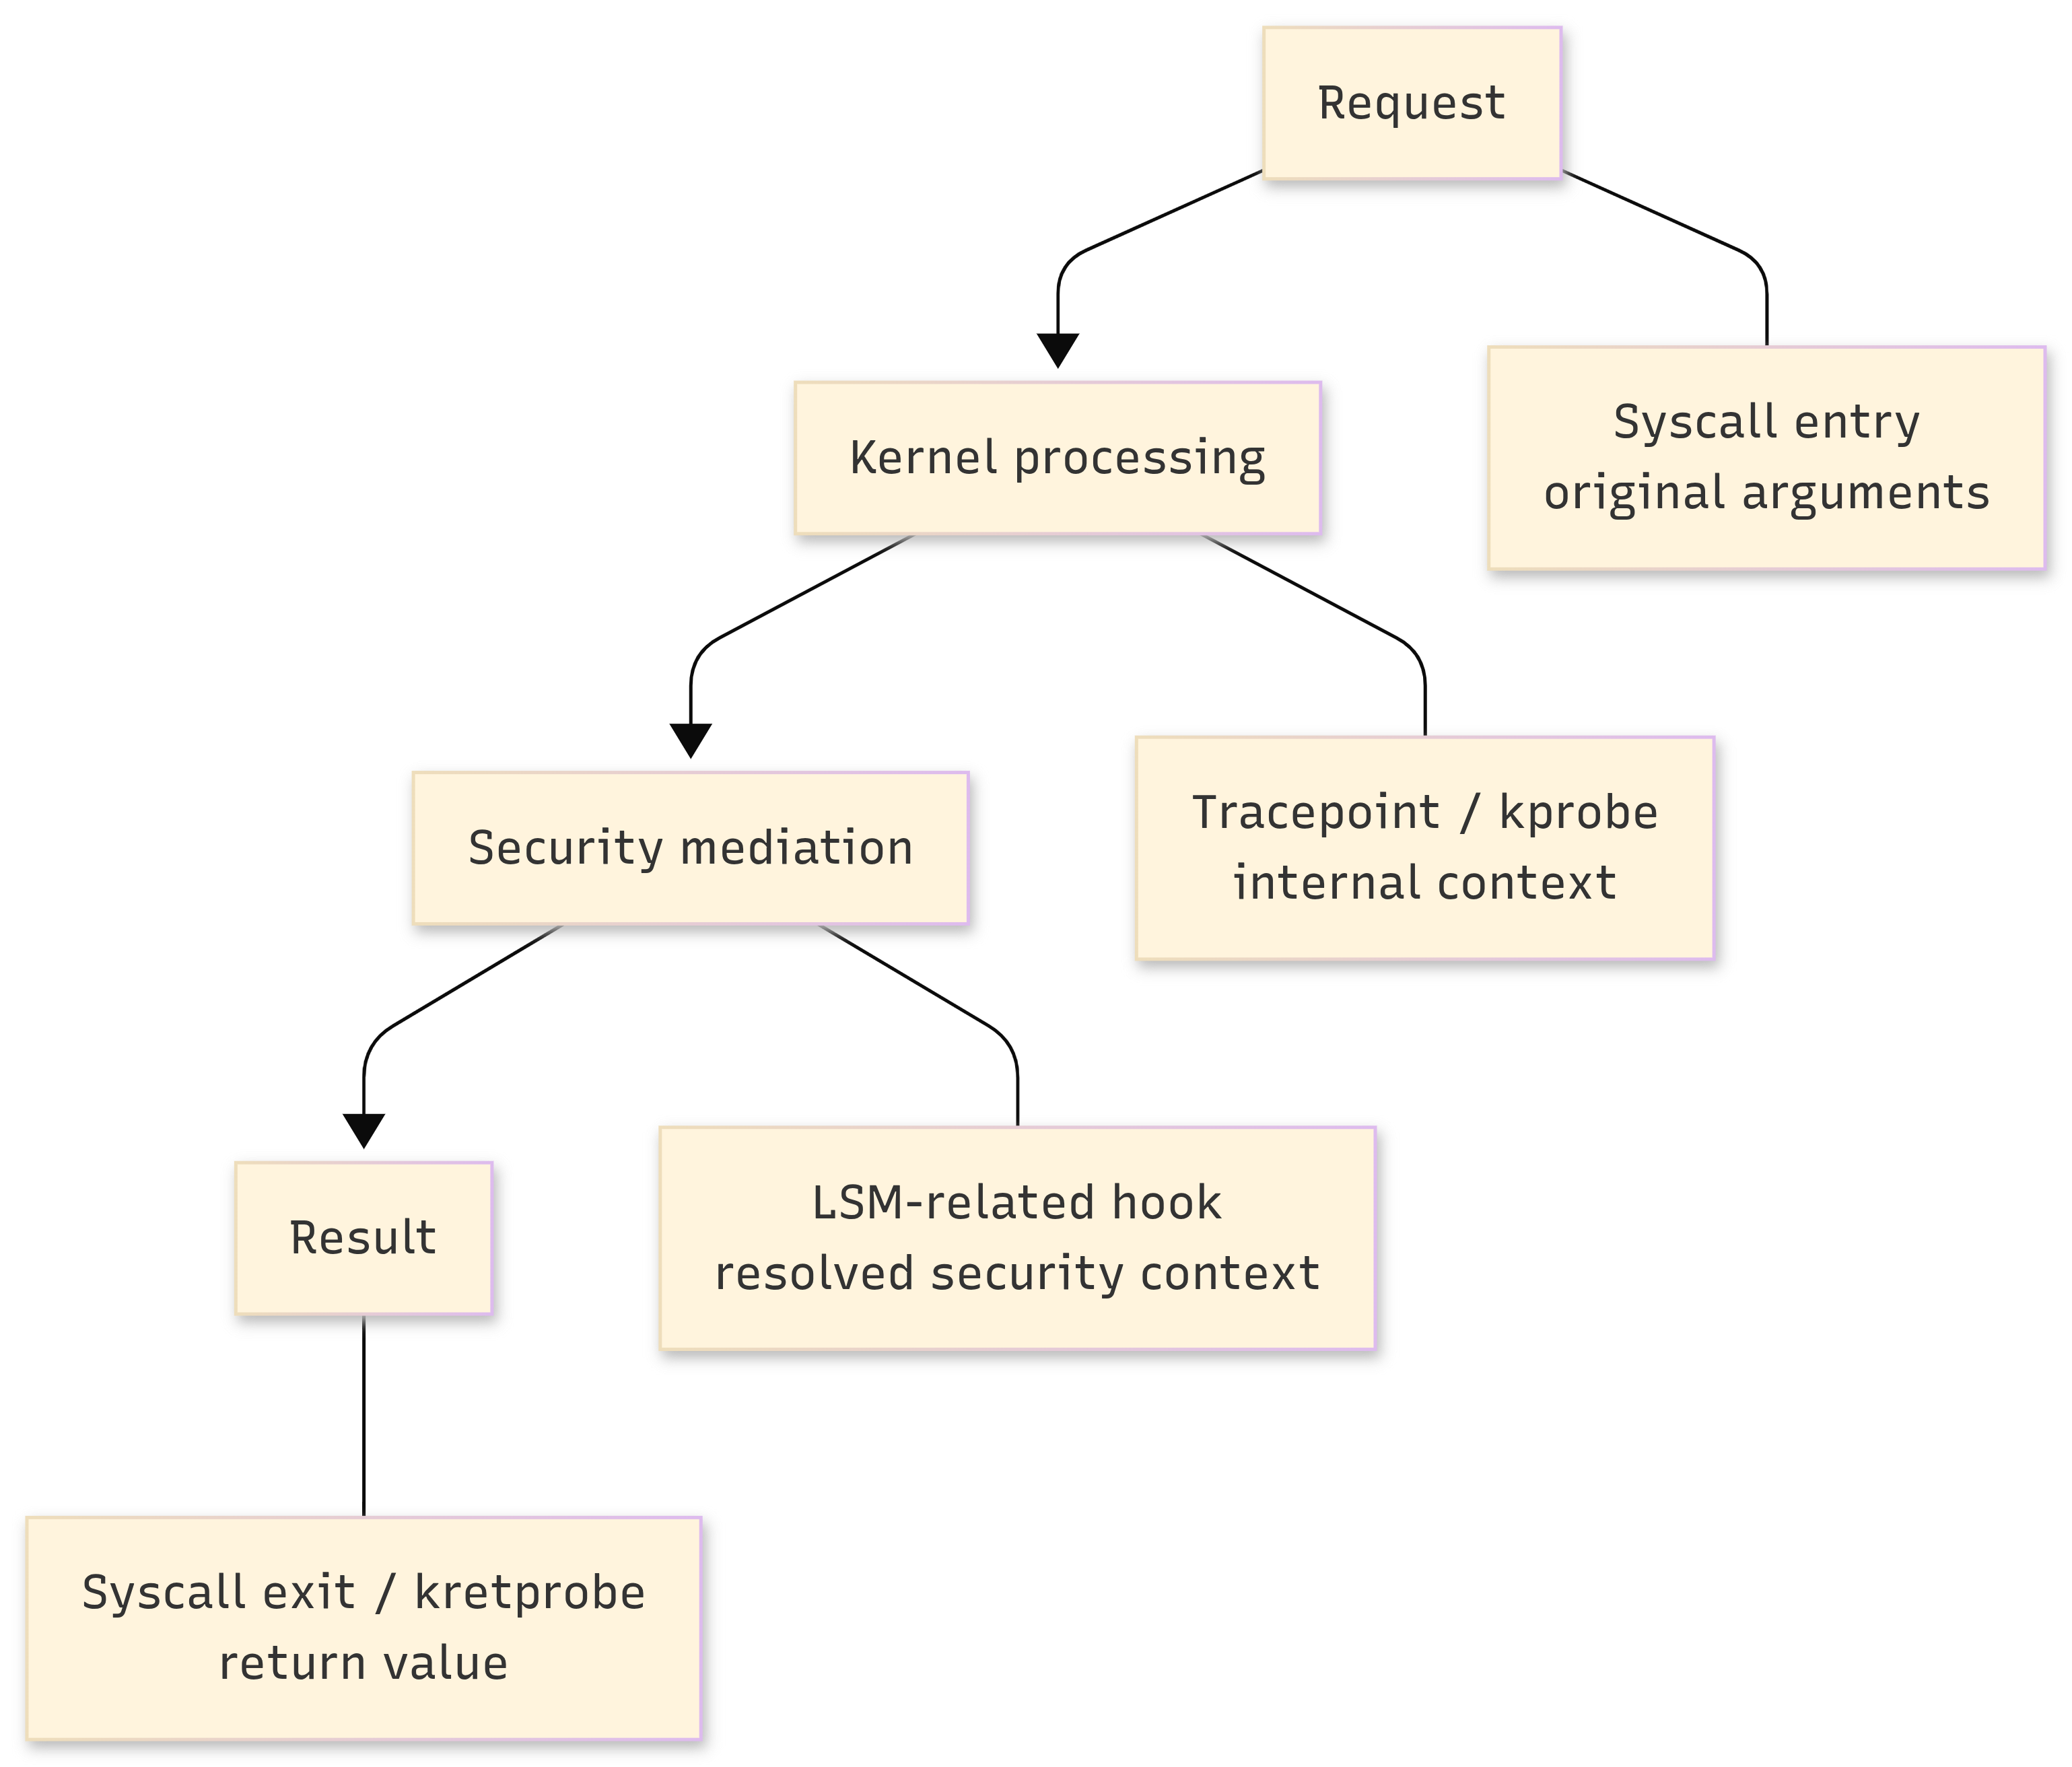
\includegraphics[
        width=0.90\textwidth,
        height=0.55\textheight,
        keepaspectratio
    ]{figures/chapter2/eBPF_observation_progression.png}

    \caption[Complementary evidence exposed by different observation points along a kernel operation.]
    {Complementary evidence exposed by different observation points along a kernel operation.}

    \label{fig:ebpf-observation-progression}
\end{figure}

\subsection{Maps, Helpers and Kernel-to-Userspace Transport}
\label{subsec:ebpf-maps-helpers-transport}

Maps are typed kernel objects through which eBPF programs store state or
exchange data with user space. Different map types provide different access
semantics, including key-value lookup, per-CPU storage, arrays, queues, and
event-oriented communication. Their key and value sizes, capacity, flags, and
lifetime are configured when the map is created. Maps make it possible to keep
configuration or short-lived state outside the limited BPF stack, but every map
operation remains subject to verifier checks and map-specific concurrency
semantics \cite{linux_bpf_maps,linux_bpf_syscall}.

Helpers are kernel functions exposed to eBPF programs through a controlled
interface. They provide operations such as obtaining process identity, reading
kernel or user memory through approved paths, accessing maps, retrieving time,
and submitting event data. Helper availability depends on the program type and
kernel version. Consequently, a helper documented for eBPF in general cannot be
assumed to be callable by every program or present on every target
\cite{linux_bpf_helpers,linux2026ebpfverifier}.

Event transport bridges the execution of short kernel programs and the more
complex processing performed in user space. A perf-event array can direct
records to per-CPU perf ring buffers, from which a consumer reads samples and
lost-event notifications. The BPF ring buffer is a separate map design with a
shared multi-producer, single-consumer buffer; among its motivations are more
efficient shared capacity and the preservation of reservation order across
CPUs. Neither mechanism provides unbounded storage. If producers outpace the
consumer or available capacity, records can be lost, so buffer sizing,
consumer throughput, and loss accounting form part of a monitor's correctness
and performance evaluation \cite{linux_perf_ring_buffer,linux_bpf_ringbuf}.

Transport choice also affects the event protocol. Kernel and user space must
agree on record framing, field widths, byte order, optional data, and event
identifiers. A successful buffer read proves only that bytes were transported;
it does not prove that they were interpreted as the event that produced them.
Stable identifiers and explicit decoding rules are therefore as important as
the selected buffer technology
\cite{gbadamosi2024ebpf,linux_perf_ring_buffer}.

\subsection{BTF and CO-RE Portability}
\label{subsec:ebpf-btf-core}

\gls{btf} represents types and related metadata in a compact format understood
by the kernel and BPF tooling. BTF may describe C types and strings and can also
carry function, line, and relocation information. When kernel BTF is available,
loaders and debugging tools can reason about kernel data structures without
depending solely on a set of headers copied from one kernel build
\cite{linux_btf}.

\gls{core} uses this type information to reduce coupling between a compiled
eBPF object and the layout of kernel data structures on the target system. The
compiler records relocation information for relevant field and type accesses;
at load time, \texttt{libbpf} compares those expectations with target BTF and
adjusts compatible accesses. This approach allows one object to tolerate
structural differences such as a field moving to another offset
\cite{linux_btf,linux_bpf_llvm_relocations,linux_libbpf_overview}.

CO-RE does not create functionality that the target kernel lacks. It cannot
provide an absent tracepoint, helper, program type, symbol, or security
permission, and it does not guarantee verifier acceptance. It addresses
structural portability, while behavioural and feature compatibility still
require explicit checks. This distinction is especially important for
enterprise distributions, which may retain an older upstream version number
while backporting selected fixes and capabilities. The effective feature set
must be established from the target kernel and distribution, not from the
version string alone \cite{linux_bpf_design_qa,redhat2025backporting}.

\section{Runtime Security and Anomaly Detection}
\label{sec:runtime-security-anomaly-detection}

Runtime security monitoring converts operating-system activity into evidence
that can support detection and investigation. An \gls{idps} may use
signature-based techniques, anomaly-based techniques, or combinations of both.
Signature-based detection compares observations with known patterns, whereas
classical anomaly detection identifies deviations from a model of expected
behaviour \cite{scarfone2007idps,chandola2009anomaly}. The detector layer
considered in this thesis is deterministic and rule-based: it does not learn a
baseline or assign statistical anomaly scores. The anomaly terminology below
describes the shape of the observations that make a rule relevant, not the
learning method used to discover them.

\subsection{Point, Contextual and Collective Anomalies}
\label{subsec:point-contextual-collective-anomalies}

Chandola, Banerjee, and Kumar distinguish point, contextual, and collective
anomalies. A point anomaly is an individual observation that is anomalous with
respect to the remaining data. A contextual anomaly is anomalous only under
particular contextual attributes, such as time or location. A collective
anomaly is a related group of observations whose joint behaviour is anomalous,
even when the individual observations may not be unusual
\cite{chandola2009anomaly}.

This taxonomy is useful for kernel telemetry. A single operation can be
security-relevant when its own attributes satisfy a sufficiently precise rule.
Other behaviours are better represented as an ordered group, for example a
credential transition followed shortly by execution or access to a sensitive
resource. Event-stream research formalises related ideas through ordered
patterns, selection strategies, and bounded temporal constraints
\cite{cugola2012processing,agrawal2008eventstreams}.

Contextual detection requires a trustworthy and sufficiently broad model of
the environment in which an event occurs. A node-local monitor can reliably use
local process identity and immediate event attributes, but it may not possess
cluster-wide workload history, organisational policy, or cross-node activity.
For that reason, the proposed work focuses on deterministic point detections
and short, locally correlated collective patterns. It does not claim
contextual anomaly detection or a general-purpose complex-event-processing
engine.

\subsection{Policies, Detectors and Alert Generation}
\label{subsec:policies-detectors-alerts}

Collection scope and detection logic answer different questions. A policy
defines which portion of the available event domain is relevant to a monitoring
scenario. It can select event families or constrain the processes whose
activity should proceed through the pipeline. A detector consumes normalised
events and evaluates a security condition. Keeping these responsibilities
separate allows the monitored event set to change without rewriting every
detection rule, and allows detector logic to evolve without placing all
analysis inside kernel programs. Similar separations between capture,
selection, and analysis appear in established runtime security systems
\cite{aquasecurity_tracee_policies,aquasecurity_tracee_detectors,
falcosecurity_falco_rules}.

A point detector evaluates one event and emits an alert when its predicates
match. A collective detector additionally needs state: it must retain enough
information to decide whether later events complete an ordered pattern.
Correlation keys constrain which observations may belong to the same sequence,
and a time window bounds how long partial matches remain relevant. These
choices reduce accidental correlation between unrelated processes, although
they do not by themselves prove that every emitted alert is malicious
\cite{cugola2012processing,agrawal2008eventstreams}.

An alert is a higher-level result derived from one or more source events. A
useful alert preserves enough provenance for an operator or downstream system
to understand the rule that matched and the evidence that triggered it.
Typical fields include detector identity, severity, source process attributes,
the relevant event arguments, and, for collective matches, the ordered event
sequence. This separation also permits raw telemetry and alert output to be
selected independently according to operational needs
\cite{scarfone2007idps,falcosecurity_falco_outputs}.

\subsection{MITRE ATT\&CK as a Classification Framework}
\label{subsec:mitre-attack-classification}

\gls{attack} organises observed adversary behaviour into tactics and
techniques. Tactics express the adversary's objective, while techniques
describe ways in which that objective may be pursued. The framework provides a
shared vocabulary for describing behaviour across detections, reports, and
security products \cite{strom2020attack,mitre2026attackresources}.

Associating detector output with ATT\&CK metadata improves the interpretability
and interoperability of alerts. It enables an analyst to relate a local rule to
a recognised behavioural category and allows downstream systems to group or
search alerts using stable identifiers. In the proposed work, the mapping is
therefore treated as part of the detector contract rather than as decorative
output. Its purpose is to make the security meaning of a match explicit and to
support structured analysis across the detector set
\cite{strom2020attack,mitre2026attackresources}.

The framework remains a classification system rather than an executable
detection language. A technique can manifest through different event
sequences, and one local observation may support several interpretations.
Detector-to-technique mappings consequently require deliberate review against
the behaviour represented by each rule \cite{strom2020attack,
mitre2026attackfaq}.

\section{Related Runtime Security Tools}
\label{sec:related-runtime-security-tools}

Open-source runtime security tools use kernel telemetry in materially different
architectures. Tracee presents a broad event pipeline with policy selection and
detectors; Falco centres its design on declarative rules over event streams;
Tetragon combines observability with hook-specific selectors and optional
in-kernel actions. They are useful architectural references, but their event
catalogues, threat models, and operational goals are not interchangeable
\cite{her2025ebpfsecuritytools}.

\subsection{Tracee}
\label{subsec:tracee}

Tracee is a Linux runtime security and observability system that represents
system calls, process lifecycle activity, file operations, networking data,
LSM-related observations, and derived security detections through a common
event abstraction. Events are grouped into categories and can be selected
individually or through sets \cite{aquasecurity_tracee,
aquasecurity_tracee_events}.

Tracee policies combine scope with rules that select the events and data of
interest. Filtering is divided between kernel and user space according to the
available event data and filter type. This architecture can avoid submitting
some irrelevant records while retaining richer processing after events reach
user space \cite{aquasecurity_tracee_policies}. Detection remains a separate
layer: current detectors declare their input events, process matching
observations, and can emit derived events. Tracee supports detector
implementations in Go and declarative YAML definitions, and detector output can
participate in the same event-oriented pipeline
\cite{aquasecurity_tracee_detectors,aquasecurity_tracee_detector_api}.

The system supports structured and human-readable output, stream routing, and
enrichment for operational use. Its breadth and mature event model make it an
important reference for separating collection, selection, detection, and
presentation \cite{aquasecurity_tracee_output}. The proposed work follows that
separation as a design pattern, but it is an independent and narrower research
prototype. It does not claim Tracee's event coverage, detector ecosystem,
forensic facilities, or functional equivalence.

\subsection{Other Relevant eBPF Security Tools}
\label{subsec:other-ebpf-security-tools}

Falco is a runtime security engine organised around rules evaluated over event
sources. Kernel system-call activity can be captured through its driver
architecture, while plugins provide additional sources. Falco rules are
declarative YAML objects containing a condition, output description, priority,
and optional reusable lists, macros, tags, and exceptions. A matching rule
produces an alert that can be routed to configured outputs
\cite{falcosecurity_falco_kernel_architecture,falcosecurity_falco_rules,
falcosecurity_falco_outputs}.

This model demonstrates the operational value of readable rules, reusable
expressions, explicit exceptions, and an alert-oriented interface. Falco also
maintains process and container context used to enrich individual events.
However, its documented rule conditions are evaluated against an incoming
event, and separate event sources are processed independently; the core rule
language is not presented as a general temporal sequence language across
heterogeneous sources \cite{falcosecurity_falco_event_sources,
falcosecurity_falco_rule_conditions}.

Tetragon combines eBPF-based observability with optional runtime enforcement.
Its tracing policies specify kernel hooks, captured arguments or return values,
and selectors that can match process, namespace, capability, workload, and
argument attributes. Supported actions can include emitting an event,
delivering a signal, or overriding a return value where the hook and kernel
support that operation \cite{cilium_tetragon_tracing_policy,
cilium_tetragon_selectors,cilium_tetragon_enforcement}.

Tetragon therefore moves more selection and potential response close to the
hook than an architecture centred on user-space detectors. It preserves
process-lifecycle context and emits structured events through its own
interfaces, but its documented tracing-policy model is principally
hook-centred rather than a general language for arbitrary temporal sequences
\cite{cilium_tetragon_events,cilium_tetragon_tracing_policy}. Its current
installation requirements also illustrate the dependence of advanced eBPF
functionality on kernel capabilities and BTF availability
\cite{cilium_tetragon_requirements}.

Together, Falco and Tetragon mark two useful boundaries for the proposed work.
Falco shows a mature single-event rule and alert model, while Tetragon shows the
advantages and platform requirements of in-kernel selectors and enforcement.
The prototype considered in this thesis instead retains enforcement outside its
scope and concentrates on local observation, normalisation, deterministic
point rules, and short process-aware collective patterns.

\section{Positioning of the Proposed Work}
\label{sec:positioning-proposed-work}

The proposed work occupies a deliberately bounded part of the Linux runtime
security design space. It targets process and host-security monitoring on Rocky
Linux 8.10 and its enterprise 4.18-based kernel. Vendor backports and
target-specific verifier behaviour make this environment more nuanced than its
upstream version number suggests, so compatibility is treated as a property to
be established on the target rather than inferred from nominal kernel age
\cite{redhat2025backporting}.

At a high level, eBPF programs collect selected kernel observations and can
apply a minimal early filter, while a Go runtime normalises the resulting event
stream. Declarative policies define the event domain, and automatically
activated YAML detectors evaluate deterministic predicates over individual
events or short ordered patterns. Collective detection is intentionally local
and bounded: it uses process identity and immediate parent information rather
than a persistent, cluster-wide process graph. Alerts preserve their source
evidence and carry ATT\&CK metadata as a common classification vocabulary.

This combination should be understood as an integration and engineering
contribution rather than a claim that its individual mechanisms are
unprecedented. Kernel event collection, declarative rules, policy-based
selection, user-space state, and ATT\&CK-labelled alerts all have established
precedents in Tracee, Falco, Tetragon, and related systems
\cite{aquasecurity_tracee_policies,aquasecurity_tracee_detectors,
falcosecurity_falco_rules,cilium_tetragon_tracing_policy}. The thesis instead
examines how these ideas can be assembled into a compact, independently
implemented pipeline under the constraints of the selected enterprise kernel.

Several boundaries remain explicit. The system is an observation and detection
prototype, not an enforcement engine. Its rules are deterministic rather than
machine-learned, its collective model covers short local sequences rather than
general contextual or cluster-wide correlation, and its implemented event
families represent selected coverage rather than complete host visibility.
Performance, compatibility, detector behaviour, and the effect of filtering
are evaluated experimentally in Chapter~5 rather than assumed from the
architecture. Possible orchestration in a wider deployment remains future
context and is not treated as a contribution of this thesis.
